%=======================================================================================%
% the main points of this introduction are 
% outline the complexity of biological systems for physicists
% 	> even though our theoretical models should preidct everything on the energy and length scales of biology we can't because of their heterogeneity.
%   > Give examples of the heterogenaity 
% Give some points on the history of molecular biophysics  
%   >  Hodgkin-Huxley Models
%   > Gramicidin 
% Point out how Cystic Fibrosis is an expression of this progression, going from genotype to phenotype using an ion channel to teach us biophysics. 
% conclusion.
\pagenumbering{arabic}
\setcounter{page}{1}
\chapter*{Foreword}
\label{chap:foreword}
\chapquote{I've never held a pipette} {}

The more I wrote of this thesis the more I found myself writing down things I wish I'd known when I first started studying biophysics. I was writing for my past self. Hence, I think the audience for this thesis would be those with a loose grasp of third year undergraduate physics. The most difficult thing for this audience will not be the mathematics or technical content herein, but rather the breadth of biochemical pre requisites to understand the scope of the contents. I have not had time to write an introduction to molecular biology, so I recommend a physics based introduction to those concepts such as those found in \cite{phillips2012}. On this note of pedagogy, some care has been taken to name certain authors to give the reader a kind of anchor to keep track of the literature. Similarly, when a technical concept is mentioned, I have searched for a useful review article, book or explainer. So please take citations as reading recommendations \cite{dawkins1989, hofstadter1999}.

\begin{figure}[h]
	\begin{center}
		\includegraphics[width=0.9\textwidth]{figures/myelin.jpg}
	\end{center}
	\captionsetup{singlelinecheck = false, justification=raggedright}
	\caption[Nerve Cross Section by David Goodsell] {\textbf{Nerve Cross Section by David Goodsell}}{David Goodsell is an artist who produces water colors cellular environments. Many of his works can be downloaded and used \href{https://pdb101.rcsb.org/sci-art/goodsell-gallery}{for free}. He has also produced many books and articles which would serve as a light, layperson friendly introduction to molecular biology \cite{goodsell2009, goodsell2018, goodsell2020}. This particular painting depicts a nerve fibre (blue) wrapped in an insulating myelin sheath (yellow). Electrical signals propagate into the page via voltage gated sodium and potassium protein ion channels at the edge of the nerve. We will discuss the discovery and details of this mechanism in the next chapter. They are critical to the development of biophysics.}
	\label{goodsell_figure}
\end{figure}

When I first started simulating them, I didn't even know what a protein was, but for the past 4 years I have been captivated by the unending complexity in biological systems. For some examples, please take this opportunity treat yourself to the fabulous work of \href {https://pdb101.rcsb.org/sci-art/goodsell-gallery}{David Goodsell} in figure \ref{goodsell_figure}. I've found that the mindset for solving biological problems feels very different to the focus we cultivate in students when they study idealised problems in mathematics and physics. The problems are more specific and the required knowledge is broader. For example, plasma physicists may use the same mathematical tools to describe materials as diverse as the dense stellar core to the sparse intergalactic nebulae. These objects span 28 orders of magnitude in density \cite{chen2018}. Would that we were so lucky in biology, where we struggle to apply same physical models to deal with phenomena across a single order of magnitude.For context of the length scales of biology, see figure \ref{length_scales} This heterogeneity means we need many hands to solve problems in biology. Note that the publications arising from this thesis have many authors. Each researcher specialises, not unlike their cells, in a specific discipline but we all work together to answer different aspects of the same biological questions.

\begin{figure}
	\begin{center}
		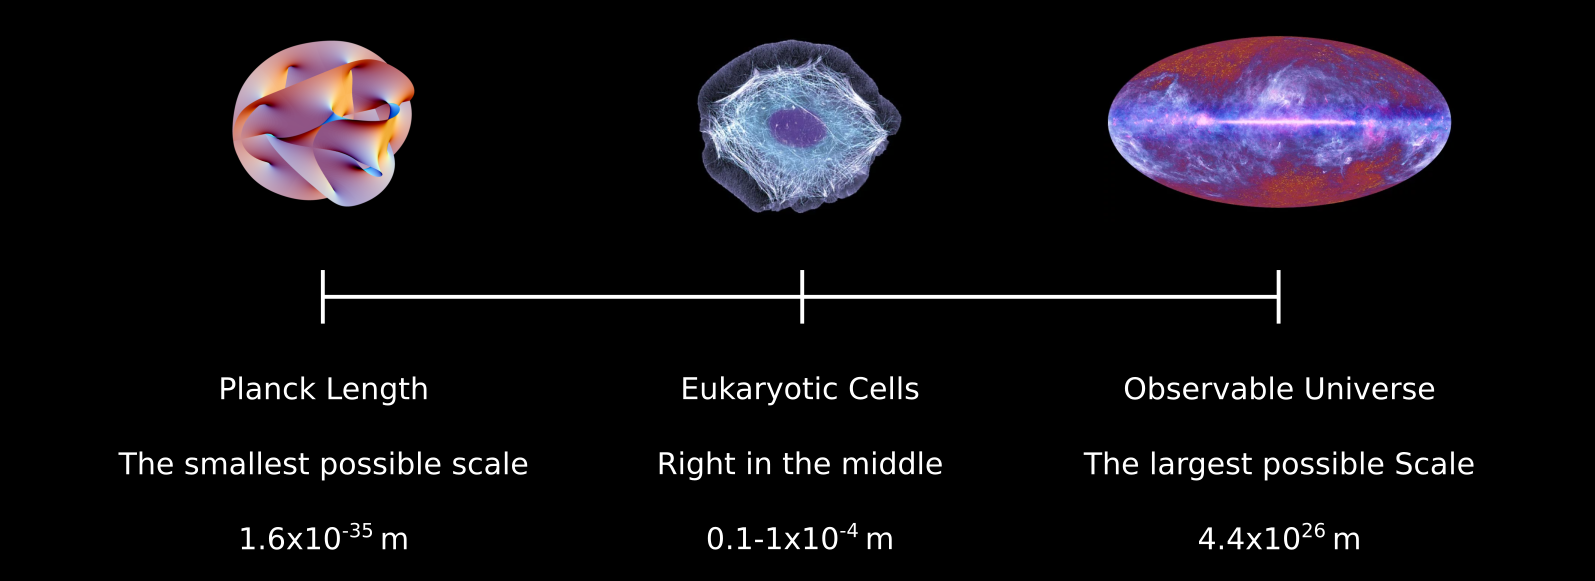
\includegraphics[width=1.0\textwidth]{figures/scales.png}
	\end{center}
	\captionsetup{singlelinecheck = false, justification=raggedright}
	\caption[The Position That Biology Occupies Compared to the Rest of Physics] {\textbf{The Position That Biology Occupies Compared to the Rest of Physics}}{It just so happens that if you plot the size of everything  in the universe on a log scale, eukaryotic cells fall right in the middle. A physicist can talk about both ends of this scale, we should learn something about the middle too.}
	\label{length_scales}
\end{figure}

Why do we need so many specially trained people to do biological research? The complexity of biology is easy to observe. If you look at your hand, you will notice hair, pores, dry skin, dead skin, perhaps even tendons and muscles twitching beneath a faint web of ghostly blood vessels. If you were to pluck a single cell from anywhere in this hierarchy and place it under an electron microscope, you would find diverse structures, called organelles. The size, shape and function of the organelles would be different if the cell was taken from somewhere else in your body. Within and between each those organelles is a wet, salty dance of molecular machines called proteins, which we will study in detail. The length scales of this journey from your arm to a single protein spans 8 orders of magnitude. At each step along the way, there are thousands of experts studying specific phenomenon at that length scale. Only by working together can these experts try to understand the whole organism.

\interfootnotelinepenalty=10000
If the reader is anything like myself they will find the amount of required knowledge to study biology a substantial barrier to entry. It is quite difficult at first to figure out what questions to ask or even figure out which subfields to study to alleviate this confusion. These challenges can be tackled by cultivating a broad coalition of connections; speak to medical doctors, clinicians, evolutionary biologists \cite{dawkins1989, dawkins2016}, philosophers, molecular biologists, biochemists\footnote{These last two are in fact different subfields but like many in this list it'll take you some time to understand the subtle differences which define each one.}, cell biologists, geneticists, bioinformaticians, theoretical chemists, computer scientists, neuroscientists, physicists, mathematicians, everyone. It will take time but remain patient and you will find that a physics motivated approach can indeed explain and eventually predict outcomes in biological experiments. A broad world view awaits you and it's really quite fun. 
%If the reader is anything like myself they will find the amount of required knowledge to study biology a substantial barrier to entry. It is quite difficult at first to figure out what questions to ask or even figure out which subfields to study to alleviate this confusion. These challenges can be tackled by cultivating a broad coalition of connections; speak to medical doctors, clinicians, evolutionary biologists \cite{dawkins1989, dawkins2016}, philosophers, molecular biologists, biochemists\footnote{These last two are in fact different subfields but like many in this list it'll take you some time to understand the subtle differences which define each one.\enlargethispage{-\baselineskip}}, cell biologists, geneticists, bioinformaticians, theoretical chemists, computer scientists, neuroscientists, physicists, mathematicians, everyone. It will take time but remain patient and you will find that a physics motivated approach can indeed explain and eventually predict outcomes in biological experiments. A broad world view awaits you and it's really quite fun. 

If this is being read by a future trainee, I hope the physics focussed philosophy in the introduction of chapter \ref{chap:intro} and the literature review of simulation techniques in chapter \ref{chap:methods} can serve as a road map, but a physicist studying biology will be best served by nurturing a strong base in electrodynamics and statistical mechanics \cite{griffiths2017, reif2009, zuckerman2010}. One particularly thorny issue is that the field is now progressing so quickly that I'm sure much of this thesis will be out of date by the time it's read by anybody I'd hope to train. But that's part of the excitement. Shoot me an email if you want help \href{mailto:miro.astore@gmailcom}{miro.astore@gmail.com}. Hopefully I'm still around.

The task head is immense. We're not exactly sure how many proteins are expressed by the human genome, but it's estimated that there are upward of 20 thousand \cite{salzberg2018}. By contrast, this thesis represents an all consuming effort by a single PhD student expending decades worth of computation time to make incremental progress in the study of a single one. There is so much to do. Good luck, and bring a towel \cite{adams1979}. 
